\documentclass[10pt,a4paper]{article}
\usepackage[T1]{fontenc}
\usepackage[utf8]{inputenc}
\usepackage{amsmath, amssymb, amsthm, thmtools, amsfonts, mathtools}
\usepackage{nicefrac}
\usepackage{calc}
\usepackage[pdftex, hyperindex, plainpages=false]{hyperref}
\usepackage[nameinlink]{cleveref} %load before classicthesis (clash)
%\usepackage[nochapters,pdfspacing]{classicthesis}
\usepackage{siunitx}
\usepackage[siunitx]{circuitikz}

\usepackage[a4paper]{geometry}
\usepackage{float}
\usepackage{mdframed}
\usepackage{titling}
\usepackage{booktabs}
\usepackage{graphicx}
\usepackage{caption, subcaption}
\usepackage{xcolor}
\usepackage[italian]{babel}
\usepackage{pgfplots}
\usepackage{listings}
%\usepackage{lmodern}
\usepackage{url}
\usepackage{enumitem}
\usepackage{tikz} %loads after classicthesis (xcolor incompat)

% lets graphicx know path where figures to be included are found
\graphicspath{{../figs/}}
\makeatletter
\def\input@path{{../figs/}}
%or: \def\input@path{{/path/to/folder/}{/path/to/other/folder/}}
\makeatother

% tikz pgf plots setup
\usepgfplotslibrary{external}
\pgfplotsset{compat=1.15}
%\tikzexternalize

% spaces and significant digits/figures for measurements
\sisetup{free-standing-units, space-before-unit, number-unit-product = \;,
scientific-notation = false, round-mode = figures, round-precision = 1,}

% turns all (hyperlinked) references black [default is blue]
\hypersetup{
	linktoc=all,
	colorlinks=true,
	linkcolor=black
}

% code listings config
%\lstset{
%language=Python,
%basicstyle=\ttfamily,
%columns=fullflexible,
%keepspaces=true,
%}

% mdframed (for boxed text) configuration
\mdfsetup{linewidth=0.6pt}

% Default fixed font does not support bold face
\DeclareFixedFont{\ttb}{T1}{txtt}{bx}{n}{12} % for bold
\DeclareFixedFont{\ttm}{T1}{txtt}{m}{n}{12}  % for normal

% Custom colors
\usepackage{color}
\definecolor{deepblue}{rgb}{0,0,0.5}
\definecolor{deepred}{rgb}{0.6,0,0}
\definecolor{deepgreen}{rgb}{0,0.5,0}

% Commands 
\newcommand{\executeiffilenewer}[3]{%
	\ifnum\pdfstrcmp{\pdffilemoddate{#1}}%
		{\pdffilemoddate{#2}}>0%
	{\immediate\write18{#3}}\fi%
}
% input .svg --> .pdf_tex graphs
%\newcommand{\includesvg}[1]{%
%	\executeiffilenewer{#1.svg}{#1.pdf}%
%	{inkscape -z -D --file=#1.svg %
%	--export-pdf=#1.pdf --export-latex}%
%	\input{#1.pdf_tex}%
%}
% Thanks UniPi's Department of Physics E. Fermi
\newcommand{\thanksdf}{(\thanks{Dipartimento di Fisica E.~Fermi,%
Universit\`a di Pisa - Pisa, Italy.}\;)}

% hyperlink to email address
\newcommand{\mail}[1]{\href{mailto:#1}{\textsf{#1}}}

% \vec for bold vectors, instead of overarrows (now "\arrvec")
\let\arrvec=\vec
\renewcommand{\vec}[1]{\boldsymbol #1}
% replaces straight phi with slanted phi
\renewcommand{\phi}{\varphi}
% replaces straight eps with curved epsilon
\newcommand{\eps}{\varepsilon}
% abbreviation for (sub_/super^)scripts of \lim, \sum,... in inline math
\newcommand{\ds}{\displaystyle}

% blackboard/number set letters
\newcommand{\CC}{\mathbb C}
\newcommand{\HH}{\mathbb H}
\newcommand{\KK}{\mathbb K}
\newcommand{\NN}{\mathbb N}
\newcommand{\PP}{\mathbb P}
\newcommand{\QQ}{\mathbb Q}
\newcommand{\RR}{\mathbb R}
\newcommand{\ZZ}{\mathbb Z}

\newcommand{\Abs}[1]{{\left\Vert #1\right\Vert}}
\newcommand{\enclose}[1]{{\left( #1 \right)}}
\newcommand{\Enclose}[1]{{\left[ #1 \right]}}
\newcommand{\floor}[1]{\left\lfloor #1 \right\rfloor}
\newcommand{\ceil}[1]{\left\lceil #1 \right\rceil}
\newcommand{\To}{\rightrightarrows}

% Math operators
\DeclareMathOperator{\divergence}{div}
\renewcommand{\div}{\divergence}
\DeclareMathOperator{\Imaginarypart}{Im}
\renewcommand{\Im}{\Imaginarypart}
\DeclareMathOperator{\Realpart}{Re}
\renewcommand{\Re}{\Realpart}
%\DeclareMathOperator{\arg}{arg}
\DeclareMathOperator{\tg}{tg}
\DeclareMathOperator{\arctg}{arctg}
\DeclareMathOperator{\settsinh}{settsinh}
\DeclareMathOperator{\settcosh}{settcosh}
\DeclareMathOperator{\tr}{tr}
\DeclareMathOperator{\im}{im}
\DeclareMathOperator{\sgn}{sgn}
\DeclareMathOperator{\diag}{diag}

\DeclarePairedDelimiter{\norm}{\lVert}{\rVert}
\DeclarePairedDelimiter{\scalar}{\langle}{\rangle}

% Logarithm with arbitrary base.
% -> log_10
\newcommand{\llog}[1][10]{\log_{#1}}

% Absolute value.
% -> |x|
\newcommand{\abs}[1]{\left| #1 \right|}

% Powers.
% -> x^a
\newcommand{\power}[2][2]{\left( #2 \right)^{#1}}

% Square.
% -> x^2
\newcommand{\sq}[1]{\power[2]{#1}}

% Expansion of the binomial coefficient.
% -> n1!/(n2!(n1 - n2)!)
\newcommand{\binomexpr}[2]{\frac{#1!}{#2!(#1 - #2)!}}

% Expression evaluation at a given point with square brackets.
% -> [x]_{a}
\newcommand{\at}[2]{\left[ #1\right]_{\makebox[-1pt][l]{${\scriptstyle#2}$}}}

% Expression evaluation in an interval.
% -> [x] _{a}^{b}
\newcommand{\eval}[3]{\left.#1%
  \right|_{\makebox[-1pt][l]{${\scriptstyle#2}$}}^{\makebox[-1pt][l]{${\scriptstyle#3}$}}}

% Upright d in math mode (for differentials).
% -> d
\newcommand{\ud}{\mathrm{d}}

% Differential.
% -> dx
\newcommand{\diff}[1][x]{\,\ud{#1}}

% Base command for defining derivatives.
% -> df/dx or d^kf/dx^k
\newcommand{\basederivative}[4][]{%
  \displaystyle%
  \ifx\\#1\\\frac{#4#2}{#4#3}%
  \else%
  \frac{#4^#1#2}{#4#3^#1}%
  \fi%
}

% Total derivative.
% -> df/dx(x) or d^kf/dx^k(x)
\newcommand{\td}[4][]{%
  \basederivative[#1]{#2}{#3}{\ud}%
  \ifx\\#4\\%
  \else%
  \mkern-4mu\left(#4\right)%
  \fi%
}

% Partial derivative.
% -> df/dx(x) or d^kf/dx^k(x)
\newcommand{\pd}[4][]{%
  \basederivative[#1]{#2}{#3}{\partial}%
  \ifx\\#4\\%
  \else%
  \mkern-4mu\left(#4\right)%
  \fi%
}

\newcommand{\intinf}{\int_{-\infty}^{\infty}\!\!\!}

\newcommand{\cinterval}[2]{\left[\, #1,~#2 \,\right]}

\newcommand{\linterval}[2]{\left[\, #1,~#2 \,\right)}

\newcommand{\rinterval}[2]{\left(\, #1,~#2 \,\right]}

\newcommand{\ointerval}[2]{\left(\, #1,~#2 \,\right)}

\newcommand{\prob}[1]{\displaystyle P\left(#1\right)}

\newcommand{\pvalue}{\emph{$p$-value}}

\newcommand{\cond}{\,|\,}

\newcommand{\expect}[1]{\displaystyle E\left[#1\right]}

\newcommand{\mom}[2][]{\displaystyle {\cal M}_{#2}\ifx\\#1\\\else(#1)\fi}

\newcommand{\momalg}[1]{\displaystyle \lambda_{#1}}

\newcommand{\momcen}[1]{\displaystyle \mu_{#1}}

\newcommand{\skewness}{\displaystyle \gamma_1}

\newcommand{\kurtosis}{\displaystyle \gamma_2}

\newcommand{\charf}[1][x]{\phi_{#1}}

\newcommand{\momgenf}[1][x]{M_{#1}}

\newcommand{\fwhm}{{\scriptstyle \textsc{FWHM}}}

\newcommand{\hwhm}{{\scriptstyle \textsc{HWHM}}}

\newcommand{\median}{\mu_{\nicefrac{1}{2}}}

\newcommand{\var}[1]{\ensuremath{\text{Var}\left(#1\right)}}

\newcommand{\cov}[2]{\ensuremath{\text{Cov}\left(#1, #2\right)}}

\newcommand{\corr}[2]{\ensuremath{\text{Corr}\left(#1, #2\right)}}

\newcommand{\like}{\mathcal L}

\newcommand{\likelihood}[2][]{\like\ifx\\#2\\\else(#2\ifx\\#1\\\else;#1\fi)\fi}

\newcommand{\chisq}{\ensuremath{\chi^2}}

\newcommand{\chisquare}[2][]{\chisq\ifx\\#2\\\else(#2\ifx\\#1\\\else;#1\fi)\fi}

\newcommand{\loglikelihood}[2][]{\log\likelihood[#1]{#2}}

\newcommand{\pdf}[3][]{#2(#3\ifx\\#1\\\else;#1\fi)}

\newcommand{\binomialpdf}[2][]{\pdf[#1]{\mathcal B}{#2}}

\newcommand{\multinomialpdf}[2][]{\pdf[#1]{\mathcal M}{#2}}

\newcommand{\poissonpdf}[2][]{\pdf[#1]{\mathcal P}{#2}}

\newcommand{\uniformpdf}[2][]{\pdf[#1]{u}{#2}}

\newcommand{\exponentialpdf}[2][]{\pdf[#1]{\varepsilon}{#2}}

\newcommand{\gausspdf}[2][]{\pdf[#1]{N}{#2}}

\newcommand{\chisquarepdf}[2][]{\pdf[#1]{\wp}{#2}}

\newcommand{\cauchypdf}[2][]{\pdf[#1]{c}{#2}}

\newcommand{\erf}[1]{\ensuremath{\text{erf}\left(#1\right)}}

\newcommand{\dccases}[4][]{#2 \ifx\\#2\\\else=\fi %
  \begin{cases}
    \displaystyle #3 & \text{per variabili discrete}\\
    \displaystyle #4 & \text{per variabili continue}#1
  \end{cases}
}
% sub/super-scriptable for all symbol as math operator 
\newcommand\Scaleforall[1]{\vcenter{\hbox{\scalefont{#1}$\forall$}}}

\DeclareMathOperator*\forevery{%
  \vphantom\sum
  \mathchoice{\Scaleforall{2}}{\Scaleforall{1.4}}{\Scaleforall{1}}{\Scaleforall{0.75}}}
\geometry{left=2cm, right=2cm, top=2cm, bottom=2cm}

% indexes subsections with letters, sections with numbers (1.a, 1.b, ...)
\renewcommand{\thesubsection}{\thesection.\alph{subsection}}

% lets graphicx know path where figures to be included are found
\graphicspath{{../figs/}}

\author{Gruppo 1.AC \\ Matteo Rossi, Bernardo Tomelleri}
\title{Es03A: Amplificatore di tensione con BJT a emettitore comune}
\begin{document}
\date{\today}
\maketitle

\setcounter{section}{0}

\section*{Misura componenti del circuito}
\begin{table}[ht]
\centering
\begin{tabular}{cccccc}
\toprule
Resistenze $[\si{\ohm}]$ & $R$ & $\sigma R$ & Capacità $[\si{\F}]$ & $C$ &
$\sigma C$ \\
\midrule
\midrule
$R_C$		  & 5.06 k	& 0.04 k	 & $C\ped{in}$  & 0.23 $\rm \mu$ & 0.01 $\rm \mu$ \\
$R_{E_p}$	  & 992		& 8      & $C\ped{out}$ & 104 n			 & 4	\\
$R_{E_q}$	  & 993		& 8      & $C_E$        & 90 $\rm \mu$	 & 5	\\
$R_{E}$		  & 496		& 4      &              &				 &		\\
$R_{1_s}$	  & 19.87 k & 0.16 k &              &				 &		\\
$R_{1_t}$	  & 50.5 k  & 8 k	 &              &				 &		\\
$R_1$		  & 70.4 k  & 0.6 k	 &              &				 &		\\
$R_2$		  & 9.93 k  & 0.08 k &              &				 &		\\
$R\ped{es_p}$ & 100.5	& 0.8    &				&				 &		\\
$R\ped{es_q}$ & 100.2	& 0.8    &				&				 &		\\
$R\ped{es}$   & 50.5	& 0.5    &				&				 &		\\
\bottomrule     
\end{tabular}
\caption{Valori di resistenza e capacità misurate per i componenti del
circuito \label{tab: rcmes}}
\end{table}
Riportiamo per completezza anche il valore calcolato della resistenza di base
\[
R_B = R_1 || R_2 = 8.70 \pm 0.07 \; \si{k\ohm}
\]
e i valori delle tensioni di alimentazione continue misurate con il multimetro
\begin{align*}
V_{CC} &= 4.99 \pm 0.03 \si{\V} \\
V_{EE} &= -4.99 \pm 0.03 \si{\V}
\end{align*}
\section{Caratterizzazione del punto di lavoro del transistor}
\subsection{Misura delle componenti quiescenti}
Con il multimetro digitale abbiamo misurato
\begin{align*}
V_{BE}^Q &= 630 \pm 4 \; \si{m\V} \\
V_{CE}^Q &= 3.67 \pm 0.03 \; \si{\V} \\
I_C^Q &= \frac{\Delta V_{R_C}}{R_C} = 1.134 \pm 0.011 \; \si{m\A} \\
\end{align*}

Prendendo come riferimento (arbitrario) il valore per la tensione di soglia
della giunzione BE $V_\gamma = 0.6 \pm 0.1 \; \si{\V}$ e come valore atteso
per la tensione al terminale di base del transistor
$\ds V\ped{B, exp} = \frac{V_{CC}}{1 + R_1/R_2}$, ci aspettiamo di trovare
\begin{align*}
V\ped{BE, exp}^Q &\approx V_\gamma = 0.6 \pm 0.1 \; \si{\V} \\
I\ped{C, exp}^Q &= \frac{V_B - V_{BE}^Q}{R_E + R_B/h_{FE}} =
1.09 \pm 0.05 \si{\m\A} \\
V\ped{CE, exp}^Q &= V_{CC} - I_C^Q(R_C + R_E) = 3.9 \pm 0.2 \; \si{\V}  
\end{align*}

\subsection{Tensioni ai terminali del BJT}
Con il multimetro digitale abbiamo misurato rispetto a $V_{EE}$
\begin{align*}
V_E &= 566 \pm 3 \; \si{m\V} \\
V_B &= 1.196 \pm 0.006 \; \si{\V} \\
V_C &= 4.23 \pm 0.03 \; \si{V} \\
\end{align*}

mentre rispetto a $GND$:
\begin{align*}
V_E &= -773 \pm 4 \; \si{m\V} \\
V_B &= -3.76 \pm 0.03 \; \si{\V} \\
V_C &= -4.39 \pm 0.03 \; \si{V} \\
\end{align*}

Come valori attesi otteniamo
\begin{align*}
V\ped{E, exp} &= R_E I_E \approx R_E I\ped{C, exp}^Q = 0.54 \pm 0.2 \; \si{\V} \\
V\ped{B, exp} &= \frac{V_{CC}}{1 + R_1/R_2} = 1.24 \pm 0.13 \; \si{\V} \\
V\ped{C, exp} &= R_C I\ped{C, exp}^Q = 5.5 \pm 0.2 \; \si{V} \\
\end{align*}
\subsection{Rigidità del partitore di tensione}
Possiamo ricavare le intensità di corrente che scorrono per le resistenze
di base a partire dalle misure precedenti
\begin{align*}
I_{R_1} = \frac{V_{CC} - V_B}{R_1} = 124.4 \pm 1.2 \; \si{\micro\A} \qquad
I_{R_2} = \frac{V_B}{R_2} = 120.4 \pm 1.3 \; \si{\micro\A} 
\end{align*}
da cui ricaviamo una stima della corrente di base
\[
I_B^Q = I_{R_1} - I_{R_2} =  4.0 \pm 1.8 \; \si{\micro\A}
\]

Per condizione di partitore di tensione ``stiff'' intendiamo:
\begin{equation}
I_B^Q \ll I_P = \frac{V_B^Q - V_{EE}}{R_B}
\end{equation}
dove abbiamo chiamato $I_P$ la corrente che approssimativamente scorre nel
partitore $R_1 + R_2$.
E, dal calcolo esplicito con i valori misurati, risulta abbastanza ben
verificata
\[
I_P = 143 \pm 5 \; \si{\micro\A} > 30 \cdot I_B^Q
.\] 

Come ulteriore conferma possiamo vedere la stessa condizione come 
$I_{R_1} \sim I_{R_2} \gg I_{B}$ o, in termini di resistenze
$R_B \ll h_{fe} R_E$ che sono entrambe soddisfatte.

Possiamo anche dare una stima del guadagno in corrente continua del transistor
\[
\beta_F = h_{FE} = \frac{I_C}{I_B} = (2.8 \pm 1.3) \times 10^{2}  
\]

\section{Risposta a segnali sinusoidali}

\subsection{Inversione di fase del segnale in uscita}
La nostra stima della frequenza per cui $A_v$(dB) = -3 dB \`e
\[
f_{1A} = 7336 \pm 6 \; \si{\Hz}
\]

\subsection{Guadagno per piccoli segnali in ingresso}
Misurando con l'oscilloscopio l'ampiezza dei segnali in ingresso $v\ped{in}$
e in uscita $v\ped{out}$ dall'amplificatore possiamo ricavare una misura del
guadagno del circuito dal rapporto $A_v = \dfrac{v\ped{out}}{v\ped{in}}$.
\begin{table}[htb]
\centering
\begin{tabular}{cccc}
\toprule
$v\ped{in}(\si{m\V})$ (nom.) & $v\ped{in} \pm \sigma(v\ped{in})$ [mV] & $v\ped{out} \pm \sigma(v\ped{out})$ [V] & $A_v \pm \sigma(A_v)$ \\
\midrule
\midrule
5 & • & • & • \\
10 & • & • & • \\
25 & • & • & •  \\
50 & • & • & • \\
75 & • & • & • \\
100 & • & • & • \\
200 & • & • & •  \\
250 & • & • & • \\
300 & • & • & • \\
400 & • & • & •  \\
\bottomrule
\end{tabular} 
\caption{Misure di guadagno al variare della tensione in ingresso
all'amplificatore \label{tab: bjtmes}}
\end{table}

Ad alta frequenza ($f \gg f_1$) la retta di best-fit al plot di Bode in 
ampiezza ha i seguenti parametri:
\[
\mathrm{intercetta} = 75.928 \pm 0.008 \;\;\;\mathrm{pendenza} = -19.6747 \pm 
0.0016 \;\;\;\mathrm{correlazione} 
= -0.997 \;\;\; \chi^2 = 1647 \;\;\; d.o.f. = 1746
\]

\begin{figure}[htb]
\centering
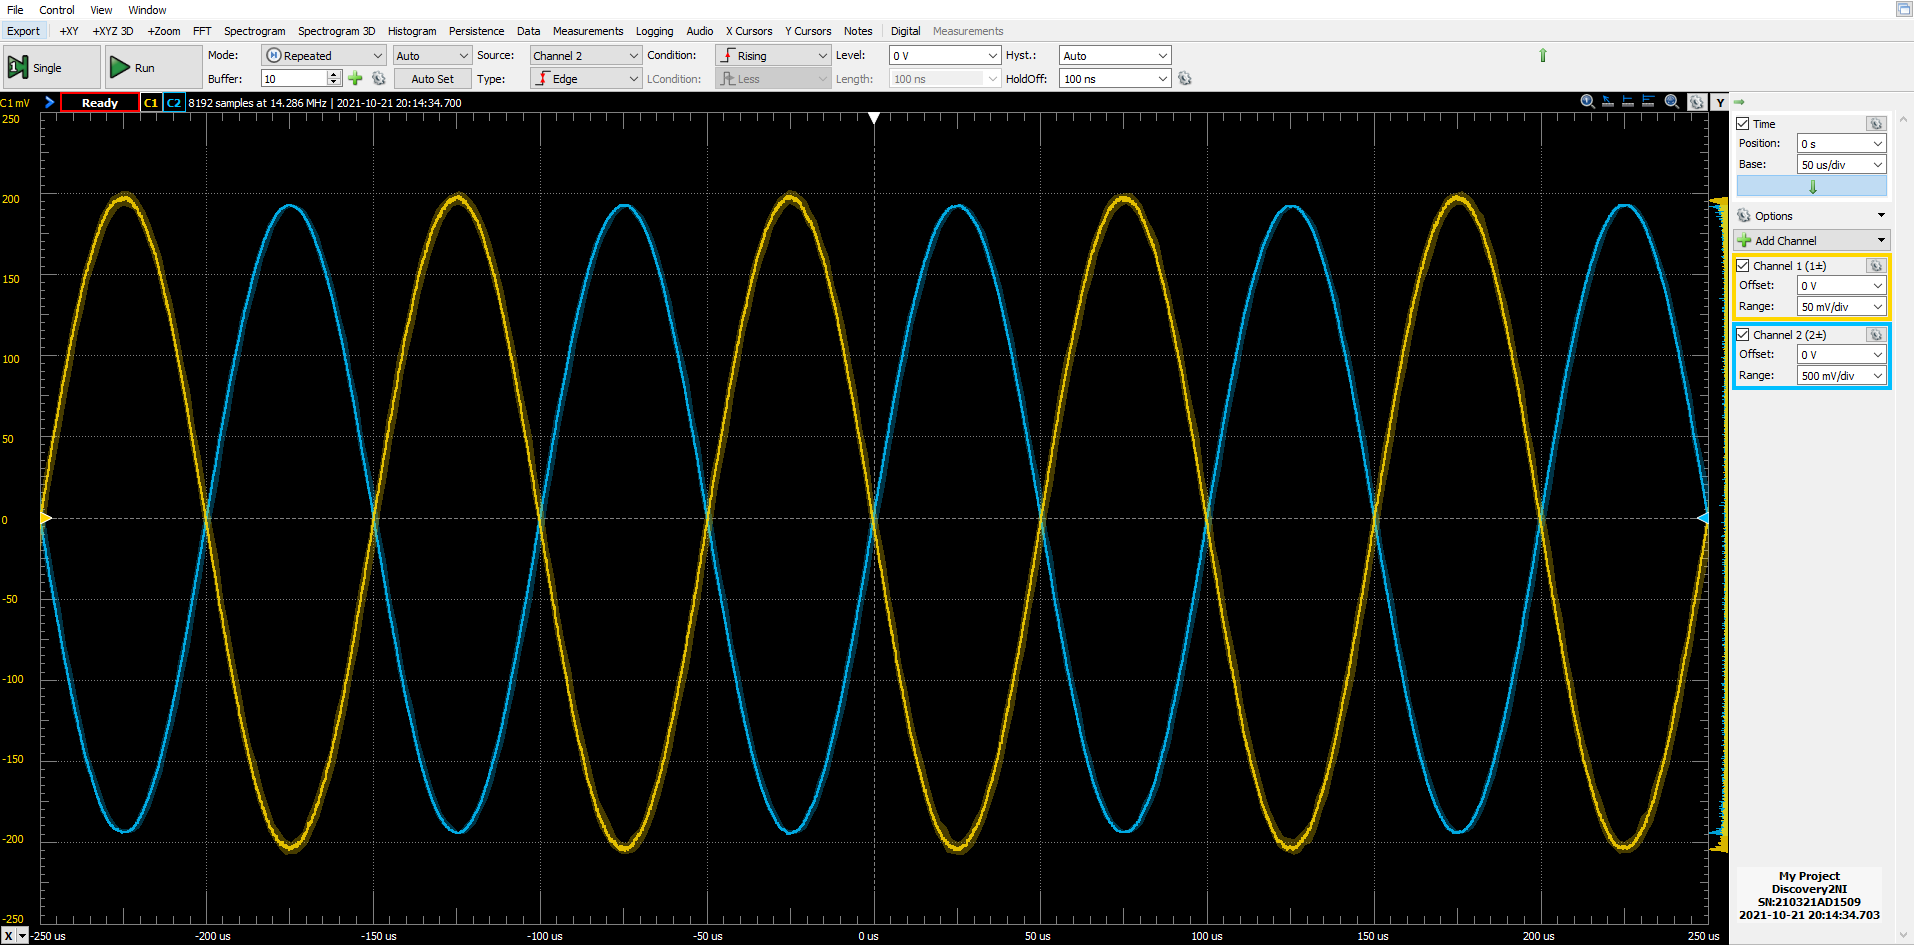
\includegraphics[scale=0.335]{Alin200mV}
\caption{Risposta del circuito ad un segnale sinusoidale di ampiezza
$\SI{200}{m\V}$ e $f = \SI{1}{k\Hz}$ in ingresso. Quando l'amplificatore
è in pieno regime attivo. \label{fig: Alin}}
\end{figure}

Il valore atteso per il guadagno dal valore dei componenti in questa
configurazione del circuito è pari a
\[
A\ped{V, exp} = -\frac{R_C}{\abs{Z_E}} = -\frac{R_C}{R_E} = -10.20 \pm 0.12
\]
Questo è compatibile con quanto trovato sperimentalmente, seppur leggermente
minore (in valore assoluto). Questo può essere spiegato da perdite dovute ai
collegamenti reali nel circuito (che trascuriamo nel modello) e
dall'indeterminazione sul valore dei parametri di costruzione del transistor.

\subsection{Linearità del circuito amplificatore}
Quando la tensione in ingresso è abbastanza alta da condurre la giunzione
BC in polarizzazione diretta il transistor entra in regime di saturazione,
dove non è più valida la relazione lineare tra le intensità di corrente di
base e collettore: per cui si osserva una distorsione del segnale in uscita.

In particolare il segnale in uscita risulta distorto o ``tosato'' in basso,
in maniera asimmetrica in corrispondenza della semionda positiva in ingresso
(per la natura invertente dell'amplificatore). Se infatti $V_{BC}$ aumenta
fino a valori prossimi a $V_\gamma$ (o perlomeno abbastanza alti da non
garantire che la giunzione BC rimanga in polarizzazione inversa) deve
diminuire $V_{CE} = V_C - V_B + V_B - V_E = -V_{BC} + V_{CE}$. Dunque ci
spostiamo a sinistra del punto di lavoro fino ad arrivare al regime di
saturazione.
Il che spiega come mai l'effetto di ``clipping'' sia più marcato durante
il semiperiodo positivo dell'onda in ingresso.

\begin{figure}[htb]
\centering
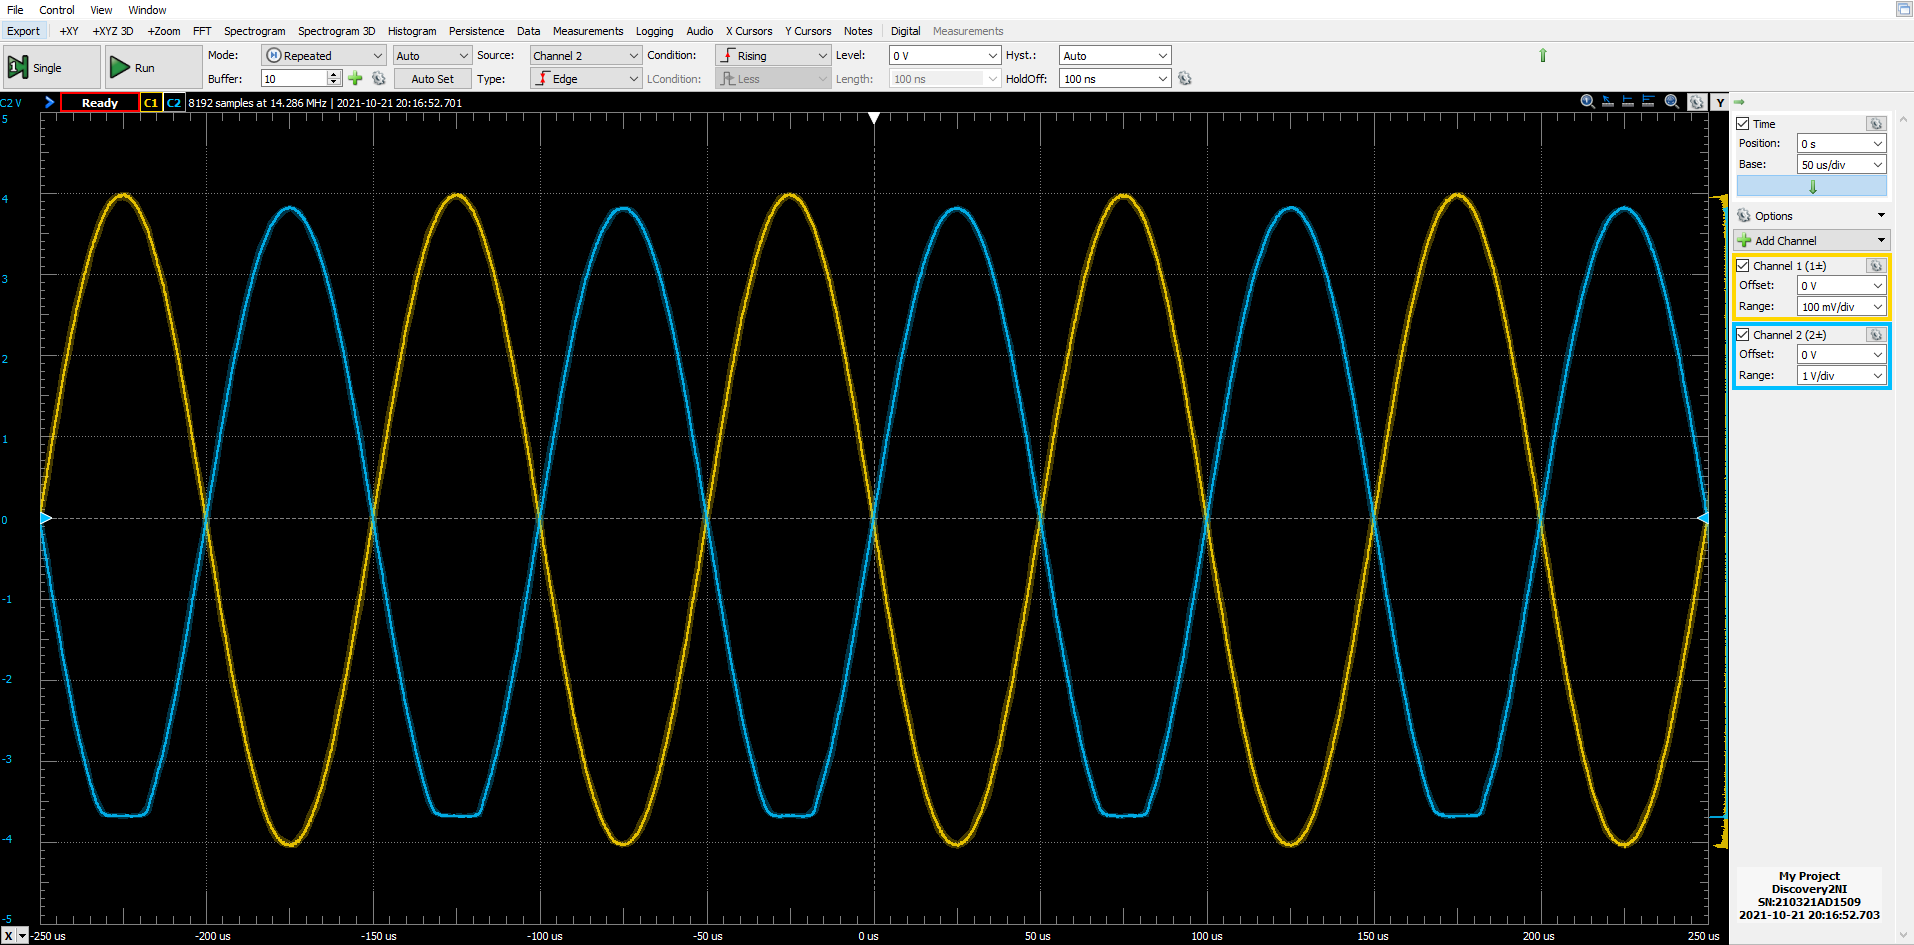
\includegraphics[scale=0.335]{Asat400mV}
\caption{Risposta del circuito ad un segnale sinusoidale di ampiezza
$\SI{450}{m\V}$ e $f = \SI{1}{k\Hz}$ in ingresso. Quando l'amplificatore
è vicino al regime di saturazione. \label{fig: Asat}}
\end{figure}


\subsection{Clipping del segnale in uscita}
Aumentando ancora l'ampiezza del segnale alternato in ingresso $v\ped{in}$ fino
a $\sim \SI{0.7}{\V}$, anche la parte alta del segnale in uscita è tagliata.
In questo caso, durante il semiperiodo negativo dell'onda in ingresso, è la
giunzione BE a cambiare polarizzazione, per cui quando entrambe le giunzioni
sono inversamente polarizzate il transistor entra in regime di interdizione.
Le uniche correnti che attraversano il BJT sono quelle di saturazione inversa,
per cui in buona approssimazione si comporta come un circuito aperto, come si
vede dal grafico delle correnti di collettore.

\begin{figure}[htb]
\centering
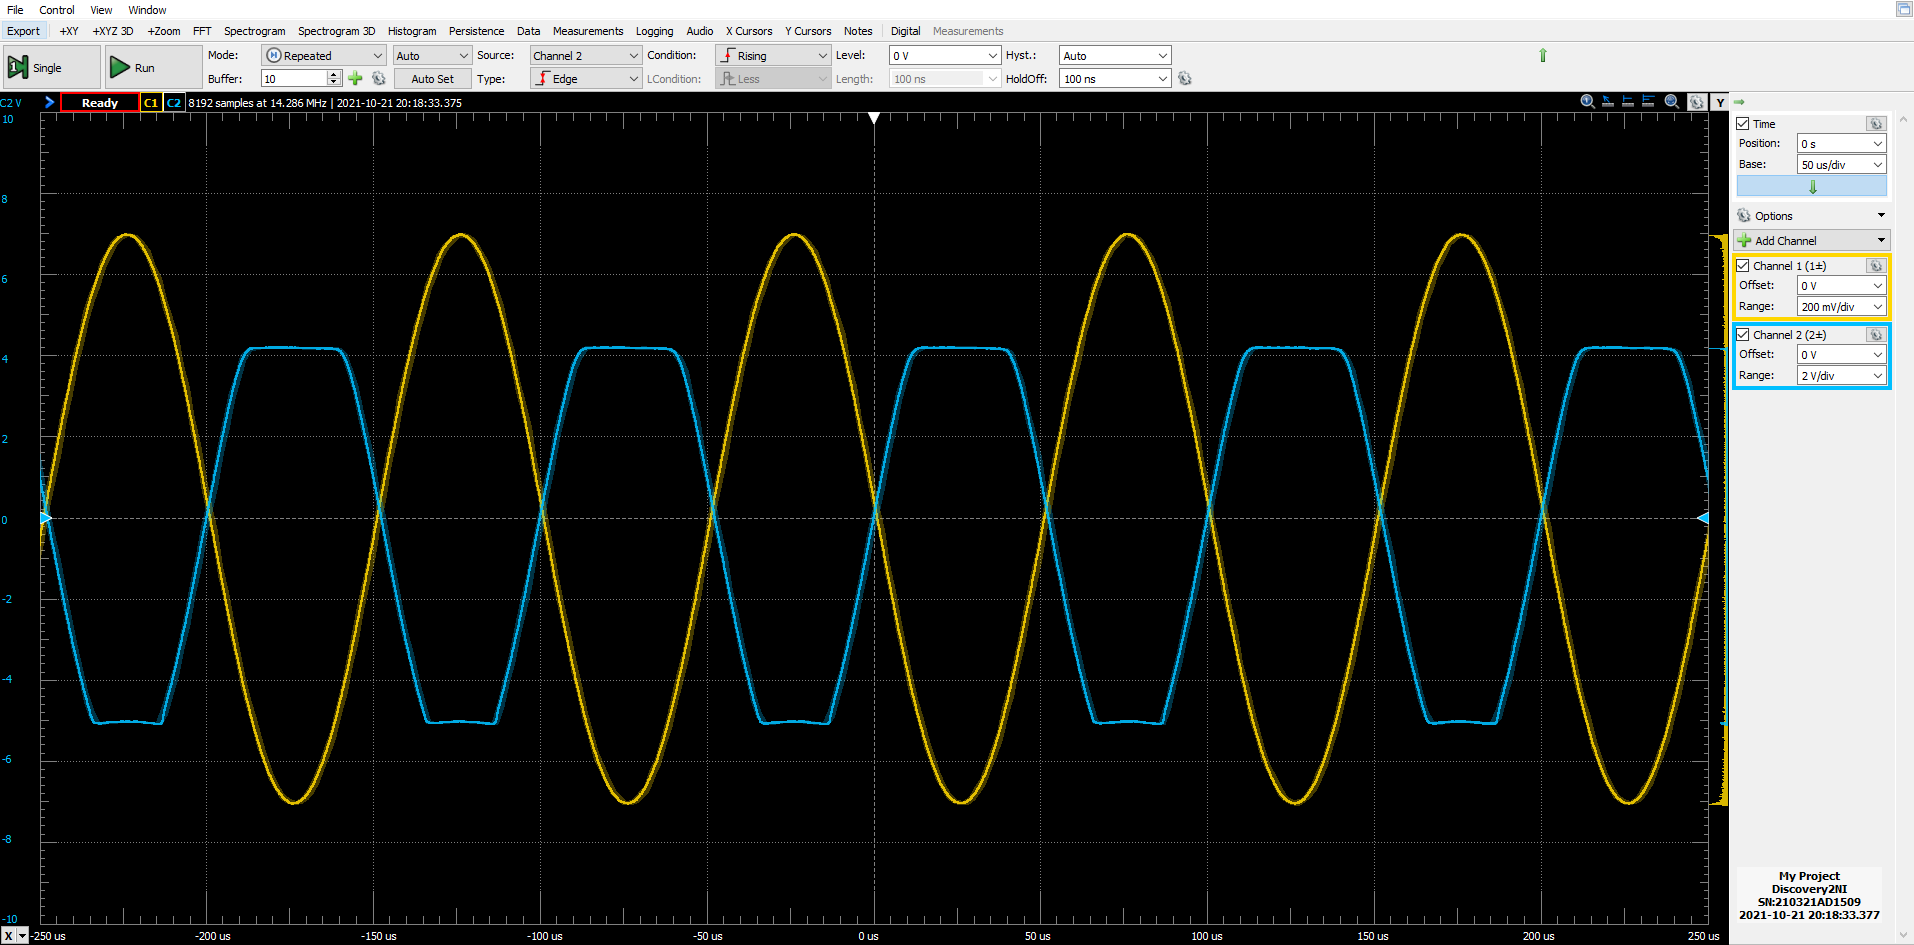
\includegraphics[scale=0.335]{Aint700mV}
\caption{Risposta del circuito ad un segnale sinusoidale di ampiezza
$\SI{700}{m\V}$ e $f = \SI{1}{k\Hz}$ in ingresso. Quando l'amplificatore
è vicino al regime di interdizione. \label{fig: Aint}}
\end{figure}

\section{Impedenze in ingresso e uscita}
\subsection{Impedenza di ingresso}
Come valore atteso per l'impedenza in ingresso al circuito abbiamo:
\[
Z\ped{in}(\omega) =
h_{ie} + h_{fe}Z_E(\omega) \; \lvert\rvert \; R_B =
\left(\frac{1}{h_{ie} + h_{fe}Z_E} + \frac{1}{R_1} + \frac{1}{R_2}\right)^{-1}
\]

dove abbiamo indicato con $Z_E(\omega)$ l'impedenza del ramo di emettitore,
che nel nostro circuito vale $Z_E = R_E$; meno che nel punto 5, dove in
parallelo a $R_E$ si aggiunge un passa alto costruito con $C_E + R\ped{es}$,
per cui vale $Z_E(\omega) = R_E || \left(R\ped{es} + \frac{1}{j \omega C_E}
\right)$.

Inserendo in serie al generatore una resistenza $R_S$ dello stesso ordine di
$R\ped{in}$ attesa e misurando la tensione in uscita con o senza $R_S$.
Detta $V_1$ la tensione $V\ped{out}$ misurata senza $R_S$ e $V_2$ la tensione
misurata con $R_S$ inserita, vale la formula:
\[
R_S/R\ped{in} = V_1/V_2 – 1
\]

\subsection{Impedenza di uscita}
Mentre come impedenza in uscita dal circuito ci aspettiamo di trovare
\[
Z\ped{out} = R_C
.\]

(Qui \`e richiesto che valutiate l'~amplificazione di centro-banda e la 
frequenza di taglio nel 
caso in cui il carico sia rispettivamente 100 e 10 k$\Omega$)
\[
\begin{array}{rl}
R_L=100 \,k\Omega & \implies A_1 = 0.98 \;\;\; f_1 = 7450 \\
R_L=10 \,k\Omega & \implies A_1 = 0.83\;\;\; f_1 = 8761 \\
\end{array}
\]

%=======================
\section{Risposta in frequenza}

\subsection{Network Analyzer}
\begin{figure}[htb]
\centering
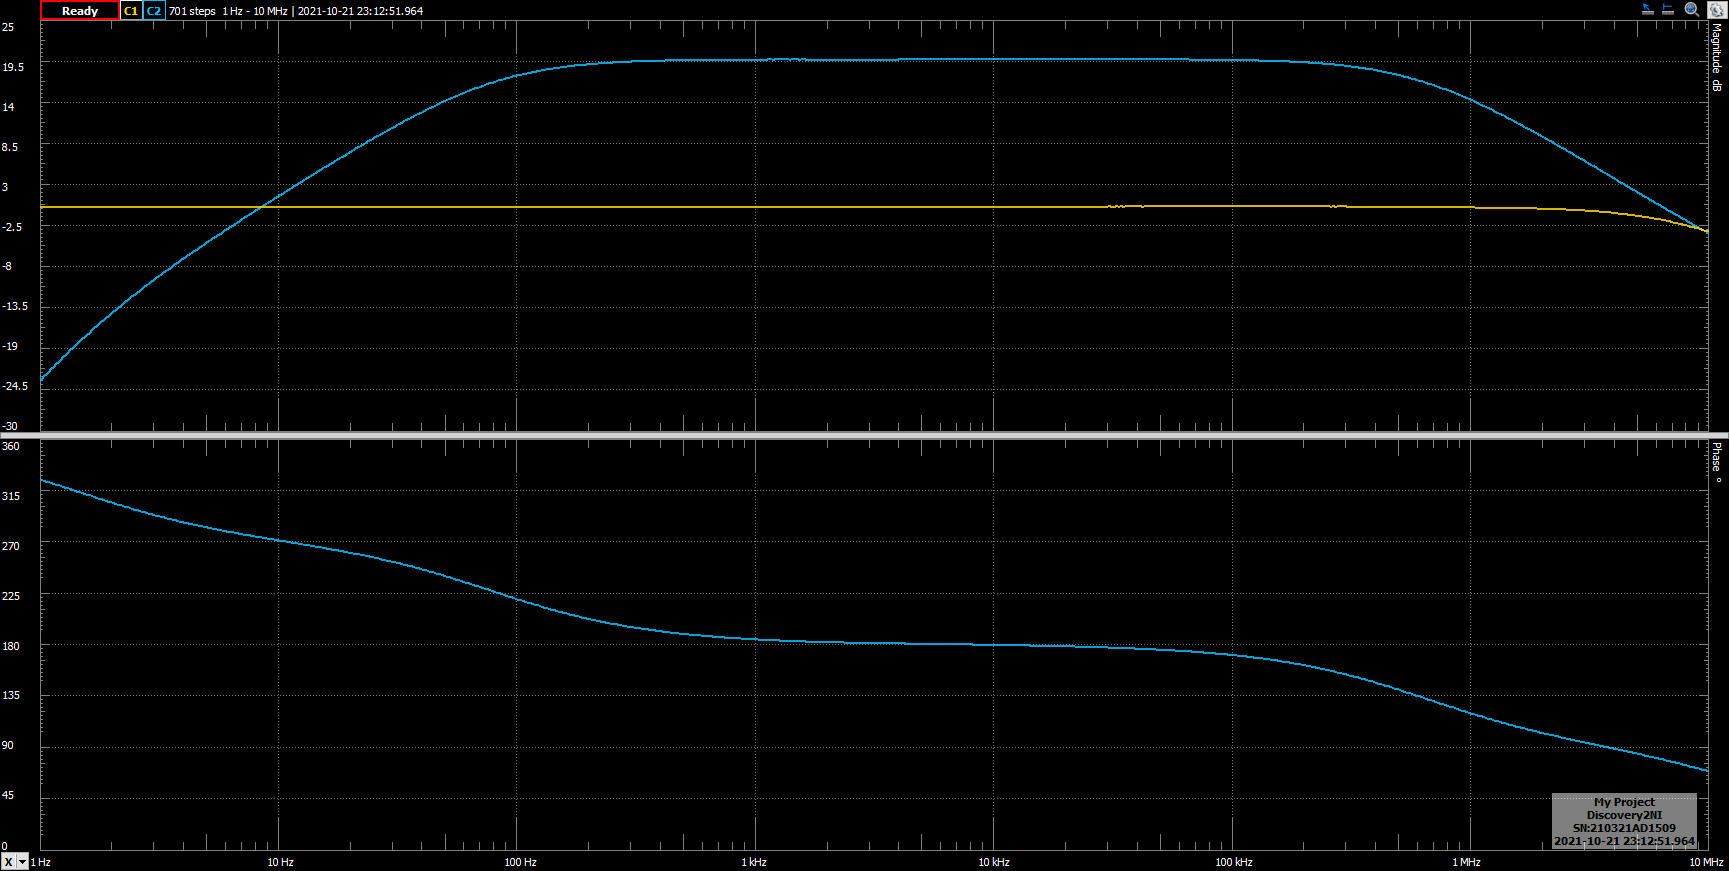
\includegraphics[scale=0.35]{1-10Mnet}
\caption{Plot di Bode ottenuto dallo scan con Network tra $1 \; \si{\Hz}$ e
$\SI{10}{M\Hz}$ con un segnale sinusoidale in ingresso di ampiezza costante
$v\ped{in} = \SI{200}{m\V}$. \label{fig: bodeplot}}
\end{figure}

\subsection{Stima delle frequenze di taglio}
Partendo da una misura con i cursori del guadagno a centro banda,
$A_V = 19.65 \pm 0.05 \; \si{dB} = 9.65 \pm 0.08$, possiamo ottenere una stima del valore
delle frequenze di taglio a bassa $f_L$ e ad alta frequenza $f_H$ dai punti
in cui il guadagno diminuisce di un fattore $1/\sqrt{2}$, cioè di circa
$-3.01 \; \si{dB}$ rispetto ad $A_V$.
\begin{align*}
f_L &= 80.77 \pm 0.12 \; \si{\Hz}\\
f_H &= 646.1 \pm 0.5 \; \si{k\Hz}
\end{align*}

Trascurando le capacità delle giunzioni nel transistor ci aspettiamo che
la frequenza di taglio ``bassa'' corrisponda a quella di un filtro passa~alto
costituito dalla serie $C\ped{in} + R_B$
\begin{equation}
f\ped{L, exp} = \frac{1}{2\pi R_B C\ped{in}} = 83 \pm 4 \; \si{\Hz}
\end{equation} 
che è in accordo con il valore misurato.

Mentre per la frequenza di taglio ``alta'' la resistenza in uscita è data
da $R_C$, per cui la capacità in serie dev'essere dell'ordine delle centinaia
di pF per avere ordine di grandezza compatibile con il valore misurato.
Ma nel datasheet risulta al massimo $C\ped{ibo} \approx \SI{25}{p\F}$, per cui
è difficile stabilire un valore di riferimento per la frequenza $f_H$ attesa.

\section{Aumento del guadagno con passa-alto all'emettitore}
Per mitigare la diminuzione del guadagno dovuta alla resistenza tra emettitore
e $V_{EE}$ si inserisce in parallelo a questa la serie $R\ped{es} + C_E$,
in modo tale che $R_E$ sia vista ``per intero'' solamente in condizioni
stazionarie (cioè dalle tensioni e correnti continue di alimentazione).
Al contrario, per frequenze abbastanza alte il condensatore si comporterà come
un corto circuito, per cui la resistenza del parallelo tenderà al valore più
piccolo tra le due resistenze, cioè $R\ped{es} \ll R_E$.
Quindi in breve l'impedenza all'emettitore si comporterà grossolanamente
come un filtro passa alto.

\subsection{Guadagno a 10 kHz con condensatore $C_E$}
Dal fit con modello la funzione di trasferimento di un filtro passa alto risulta:
\begin{figure}[htb]
\centering
%\includegraphics[scale=0.4]{passa_alto}
\caption{Fit con il modello della funzione di trasferimento per il filtro passa alto}
\end{figure}
Il valore della frequenza di taglio ricavata dal fit vale:
\begin{align*}
f_2 = 821.3 \pm 0.2 \; \si{Hz}
\end{align*}
Il guadagno a centro banda vale:
\begin{align*}
A_2 = (-25 \pm 61) \times 10^{-3} \; \si{dB}
\end{align*}
\subsection{Confronto con il guadagno atteso}
Una volta inserito il ramo in parallelo a $R_E$, dalla formula per il guadagno
atteso otteniamo
\[
A_v = -\frac{R_C}{\abs{Z_E}} =
- \frac{R_C}{R_E \; \lvert \rvert \; \left(R\ped{es} + \abs{1/j\omega C_E}
\right)} =
- R_C \abs{\frac{1}{R_E} + \frac{1}{R\ped{es} + 1/\omega C_E}}
\]

Visto che abbiamo scelto $C_E \gg C\ped{in} \sim C\ped{out}$, alla frequenza
di lavoro $f = \SI{10}{k\Hz}$ possiamo considerare trascurabile l'impedenza
del condensatore $\abs{Z_{C_E}} = \dfrac{1}{2\pi f C_E} \approx 0.1 \si{\ohm}
\ll R\ped{es}$, per cui in buona approssimazione ci aspettiamo
\[
\abs{A_v} \approx
\frac{R_C}{R_E \; \lvert \rvert \; R\ped{es}} =
R_C \abs{\frac{1}{R_E} + \frac{1}{R\ped{es}}} \approx
\frac{R_C}{R\ped{es}} = 110 \pm 1
\]

Questo però assumendo che l'impedenza del transistor sia trascurabile rispetto
a $Z_E$, o meglio $\abs{Z_E \gg \dfrac{h_{ie}}{h_{fe}}}$
\begin{align*}
\abs{Z_E} &= \abs{\frac{1}{R_E} + \frac{1}{R\ped{es} + 1/\omega C_E}}^{-1} =
45 \pm 2 \; \si{\ohm} \\
\frac{h_{ie}}{h_{fe}} &\approx \SI{40}{\ohm}
\end{align*}
che non risulta affatto verificata.

Considerando nel modello anche l'impedenza in ingresso del transistor in
serie a quella del ramo $Z_E$ avremo come valore atteso per il guadagno
\begin{equation}
A_v = \frac{R_C}{\abs{Z_E} + h_{ie}/h_{fe}} \approx 60
\end{equation}

\iffalse
\subsection*{10.c Differenze}
A differenza dei circuiti RC studiati prima, non possiamo considerare
indipendenti i sotto-circuiti che compongono il passa-banda; infatti il
comportamento reale del circuito è sensibilmente diverso da quanto previsto in 
approssimazione di stadi indipendenti.

In particolare a centro banda (i.e. nell'intervallo di frequenza
$f_2 \leq f \leq f_1$) l'attenuazione non è più in ottima approssimazione
unitaria, ma è minore di $A\ped{max}(f) \approx \SI{-6}{\dB/dec}$.

Le frequenze di taglio misurate $f_L$ e $f_H$ non sono compatibili con quelle
ottenute separatamente nell'analisi dei singoli circuiti. Più precisamente
la frequenza più bassa (del passa alto) è pressoché dimezzata
$f_L > f_2$, mentre la frequenza più alta (del passa basso) è più che
raddoppiata $f_H > f_1$.

D'altra parte, una ragionevole richiesta per assicurare l'indipendenza dei due
circuiti collegati in serie è che si abbia
$\abs{Z\ped{out, 1}} \ll \abs{Z\ped{in,2}}$ ad ogni frequenza (e 
indipendentemente da questa). Riportiamo le impedenze in questione:
\[
\abs{Z\ped{out, 1}} = \abs{\frac{R_1}{1 + j \omega R_1 C_1}}^2 = 
\frac{R_1^2}{1 + \omega^2 R_1^2 C_1^2}
\qquad
\abs{Z\ped{in, 2}}^2 = \abs{\frac{1 + j \omega R_2 C_2}{j\omega 
C_2}}^2 = \frac{1 + \omega^2 R_2^2 C_2^2}{\omega^2 C_2^2}
\]
Ora $\abs{Z\ped{out, 1}} \leq 1/(\omega C_1)$ con $\abs{Z\ped{out, 
1}} \sim 1/(\omega C_1)$ per $f \gg f_1 $ e $\abs{Z\ped{in, 2}} 
\geq 1/(\omega C_2)$ con $\abs{Z\ped{out, 1}} \sim 1/(\omega C_2) 
$ per $ f \ll f_2 $. Quindi per poter considerare indipendenti i due circuiti
è sicuramente una buona idea imporre la condizione
\[
\abs{Z\ped{out, 1}} \leq \frac{1}{\omega C_1} \ll \frac{1}{\omega C_2} \leq 
\abs{Z\ped{in, 2}} \implies C_2 \ll C_1.
\]
Mentre per i valori di capacità scelti vale la condizione opposta
$C_2 \approx 10 \cdot C_1$.

\subsection*{10.d Dipendenza dai valori delle resistenze}
Se indichiamo con $A_1(f)$ e $A_2(f)$ le attenuazioni del passa-basso e del
passa-alto, l'attenuazione attesa in uscita dai due circuiti collegati in
cascata è
\begin{equation}\label{eq: bpfgain}
A = \left(\frac{R_1}{R_2} + \frac{1}{A_1 A_2}\right)^{-1} = 
\frac{A_1 A_2}{A_1 A_2 \frac{R_1}{R_2} + 1} 
\end{equation}
Nel nostro caso vale $R_1 = R_2$ (entro l'incertezza) per cui come
attenuazione di centro banda, dove avevamo $A_1 \approx A_2 \approx 1$, ci
aspettiamo di avere $A\ped{cb} = \frac{1}{2}$.
Questo è compatibile con il valore che abbiamo misurato (prima in dB)
$A\ped{cb} = 0.4702 \pm 0.0004 \approx \frac{1}{2}$

Per avere una risposta in frequenza del circuito complessivo il più possibile
uguale al prodotto delle funzioni di trasferimento dei due sotto-circuiti
avremmo dovuto scegliere $R_1 \ll R_2$ ($Z\ped{out, 1} \ll Z\ped{in, 2}$.
Infatti l'attenuazione attesa a centro banda vista in \eqref{eq: bpfgain}
sotto queste ipotesi diventa $A\ped{cb} \approx A_1 A_2 \approx 1$.
\subsection*{10.e Andamento della fase}
Idealmente, se la funzione di trasferimento complessiva $T(\omega)$ per il
passa banda è il prodotto delle funzioni di trasferimento dei due circuiti in
cascata:
\begin{align*}
T_1(\omega) = -\frac{1}{1 + j \omega/\omega_1} \qquad
T_2(\omega) = \frac{1}{1 - j \omega_2/\omega}
\end{align*}
ci aspettiamo (per le regole di moltiplicazione sui complessi) che lo
sfasamento totale in uscita sia pari alla somma degli sfasamenti prodotti dai
singoli sotto-circuiti:
\[
T(\omega) = T_1(\omega) T_2(\omega) =
\abs{T_1} e^{i (\omega t + \phi_1)} \abs{T_2} e^{i (\omega t + \phi_2)} =
\abs{T_1} \abs{T_2} e^{i (\omega t + \phi_1 + \phi_2)} =
\abs{T_1} \abs{T_2} e^{i (\omega t + \phi)}
\]
per cui $\phi = \phi_1 + \phi_2 =
\tan^{-1} \left( \dfrac{\Im{\{T_1(\omega)\}}}{\Re{\{T_1(\omega)\}}} \right) +
\tan^{-1} \left( \dfrac{\Im{\{T_2(\omega)\}}}{\Re{\{T_2(\omega)\}}} \right)$
che corrispondono rispettivamente a
\begin{align*}
\phi_1(\omega) = \arctan - \frac{\omega}{\omega_1} \qquad
\phi_2(\omega) = \arctan \frac{\omega_2}{\omega}
\end{align*}

Effettivamente le misure di sfasamento in uscita dal passa-banda risultano
in accordo con l'andamento atteso
\begin{equation}
\phi_2 + \phi_1 = \phi(f) = \arctan{\frac{f_2}{f}} - \arctan{\frac{f}{f_1}}
\end{equation}
\begin{figure}[htb]
\centering
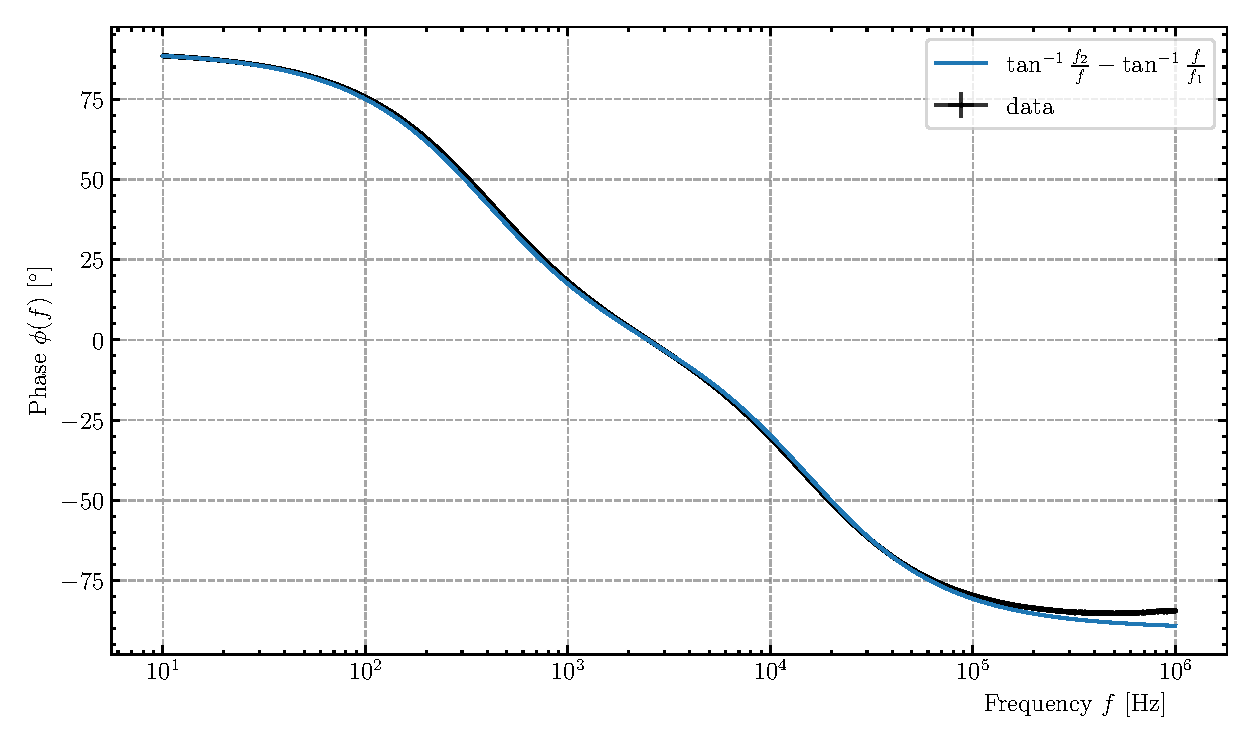
\includegraphics[scale=0.7]{bpfphase}
\caption{Grafico dello sfasamento misurato per il filtro passa-banda al
variare della frequenza in scala semilogaritmica.}
\end{figure}
almeno fino a frequenze dell'ordine di $10^5 \; \si{\Hz}$ dove i punti
iniziano a deviare dal modello man mano che ci si avvicina alla banda
passante dell'AD2 $(\sim 9 \; \si{M\Hz})$. Questo può essere dovuto alle
capacità parassite tra i fili, i componenti e la basetta che ad alta
frequenza non sono trascurabili, a differenza di quanto presuppone il nostro
modello.
\fi

\section*{Conclusioni e commenti finali}
Si è riusciti a costruire e caratterizzare un amplificatore di tensione
invertente con un BJT in configurazione di emettitore comune. In particolare
si è riusciti ad apprezzare il differente comportamento (anche non lineare)
del circuito in vari regimi, dare una stima di guadagno, impedenza di
ingresso e uscita e frequenze caratteristiche della sua risposta in frequenza.

\section*{Dichiarazione}
I firmatari di questa relazione dichiarano che il contenuto della relazione \`e
originale, con misure effettuate dai membri del gruppo, e che tutti i firmatari
hanno contribuito alla elaborazione della relazione stessa.

\end{document}
